\documentclass[12pt,a4paper]{report}

\usepackage[utf8]{inputenc}
\usepackage[T1]{fontenc}
\usepackage[english]{babel}
\usepackage[top=1cm,bottom=2cm,left=1cm,right=1cm]{geometry}
%\usepackage{url}
%\usepackage{fancyhdr}
\usepackage{sectsty}
\usepackage{wrapfig}
\usepackage{titlesec}
\usepackage{setspace}
\usepackage{graphicx}
\usepackage{lmodern}
\usepackage{url}
\usepackage{amsmath}
\usepackage{amssymb}
\usepackage{mathrsfs}
\usepackage{fancyhdr}
\usepackage{gensymb}
\usepackage{enumerate}
\usepackage{caption}
\usepackage{hyperref} % Créer des liens et des signets 
\usepackage[cc]{titlepic}
\usepackage{listing}


\title{
\rule{15cm}{1pt} \\
\Large {\bfseries Sensation and percetion} \\
\Large {\bfseries Assignement 4}\\
\rule{15cm}{1pt}}
\author{Sami Sellami}

\titlepic{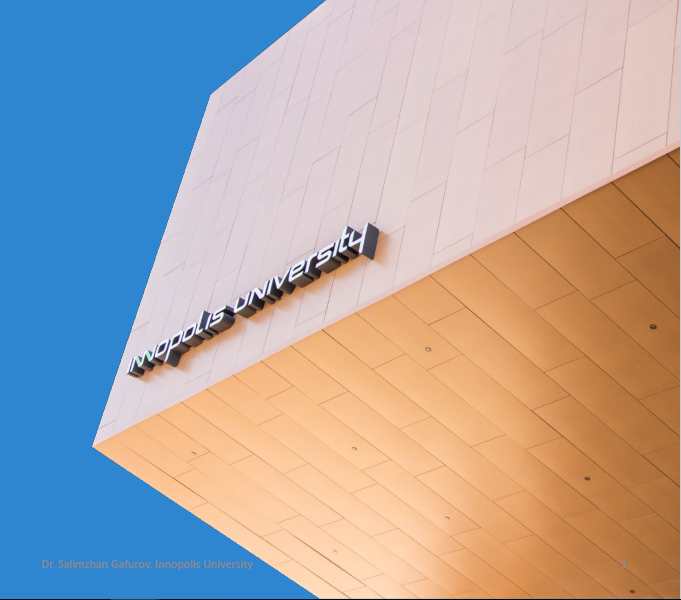
\includegraphics[width=15cm]{Innopolis_image.png}} 
\date{\today}

\begin{document}
\pagenumbering{arabic}
\setcounter{page}{1}
\setcounter{secnumdepth}{1}
	
\fontfamily{ptm}\selectfont

\maketitle

\titlelabel{\thetitle)\quad}
\titlespacing{\chapter}{0cm}{0cm}{0cm}
\titlespacing{\section}{0.2cm}{0cm}{0cm}

\textbf{NB:THE SOURCE CODE IS ATTACHED TO THE PRESENT FILE} 


\subsection{TASK 1: Color sensor unsing Arduino:}

\subsection*{Introduction:}
The task is to build a hardware, program and implement a suitable code, for a simple color sensor suitable for an application of interest. 
We are going to use an RGB LED and a Cds photocell as a colour sensor for a micro-controller. we will show  how  can we verify the colour being scanned with a small Processing sketch.

\begin{enumerate}
\item \textbf{Hardware}:

For this task we need the following equipments;
\begin{itemize}
\item Arduino microcontroler
\item Three RGB LEDs  Red Green and Blue 
\item $10k \ohm$ resistor and $1k \ohm$ resistor
\item Breadboard wires
\item A CdS photocell   
\end{itemize}

\begin{center}
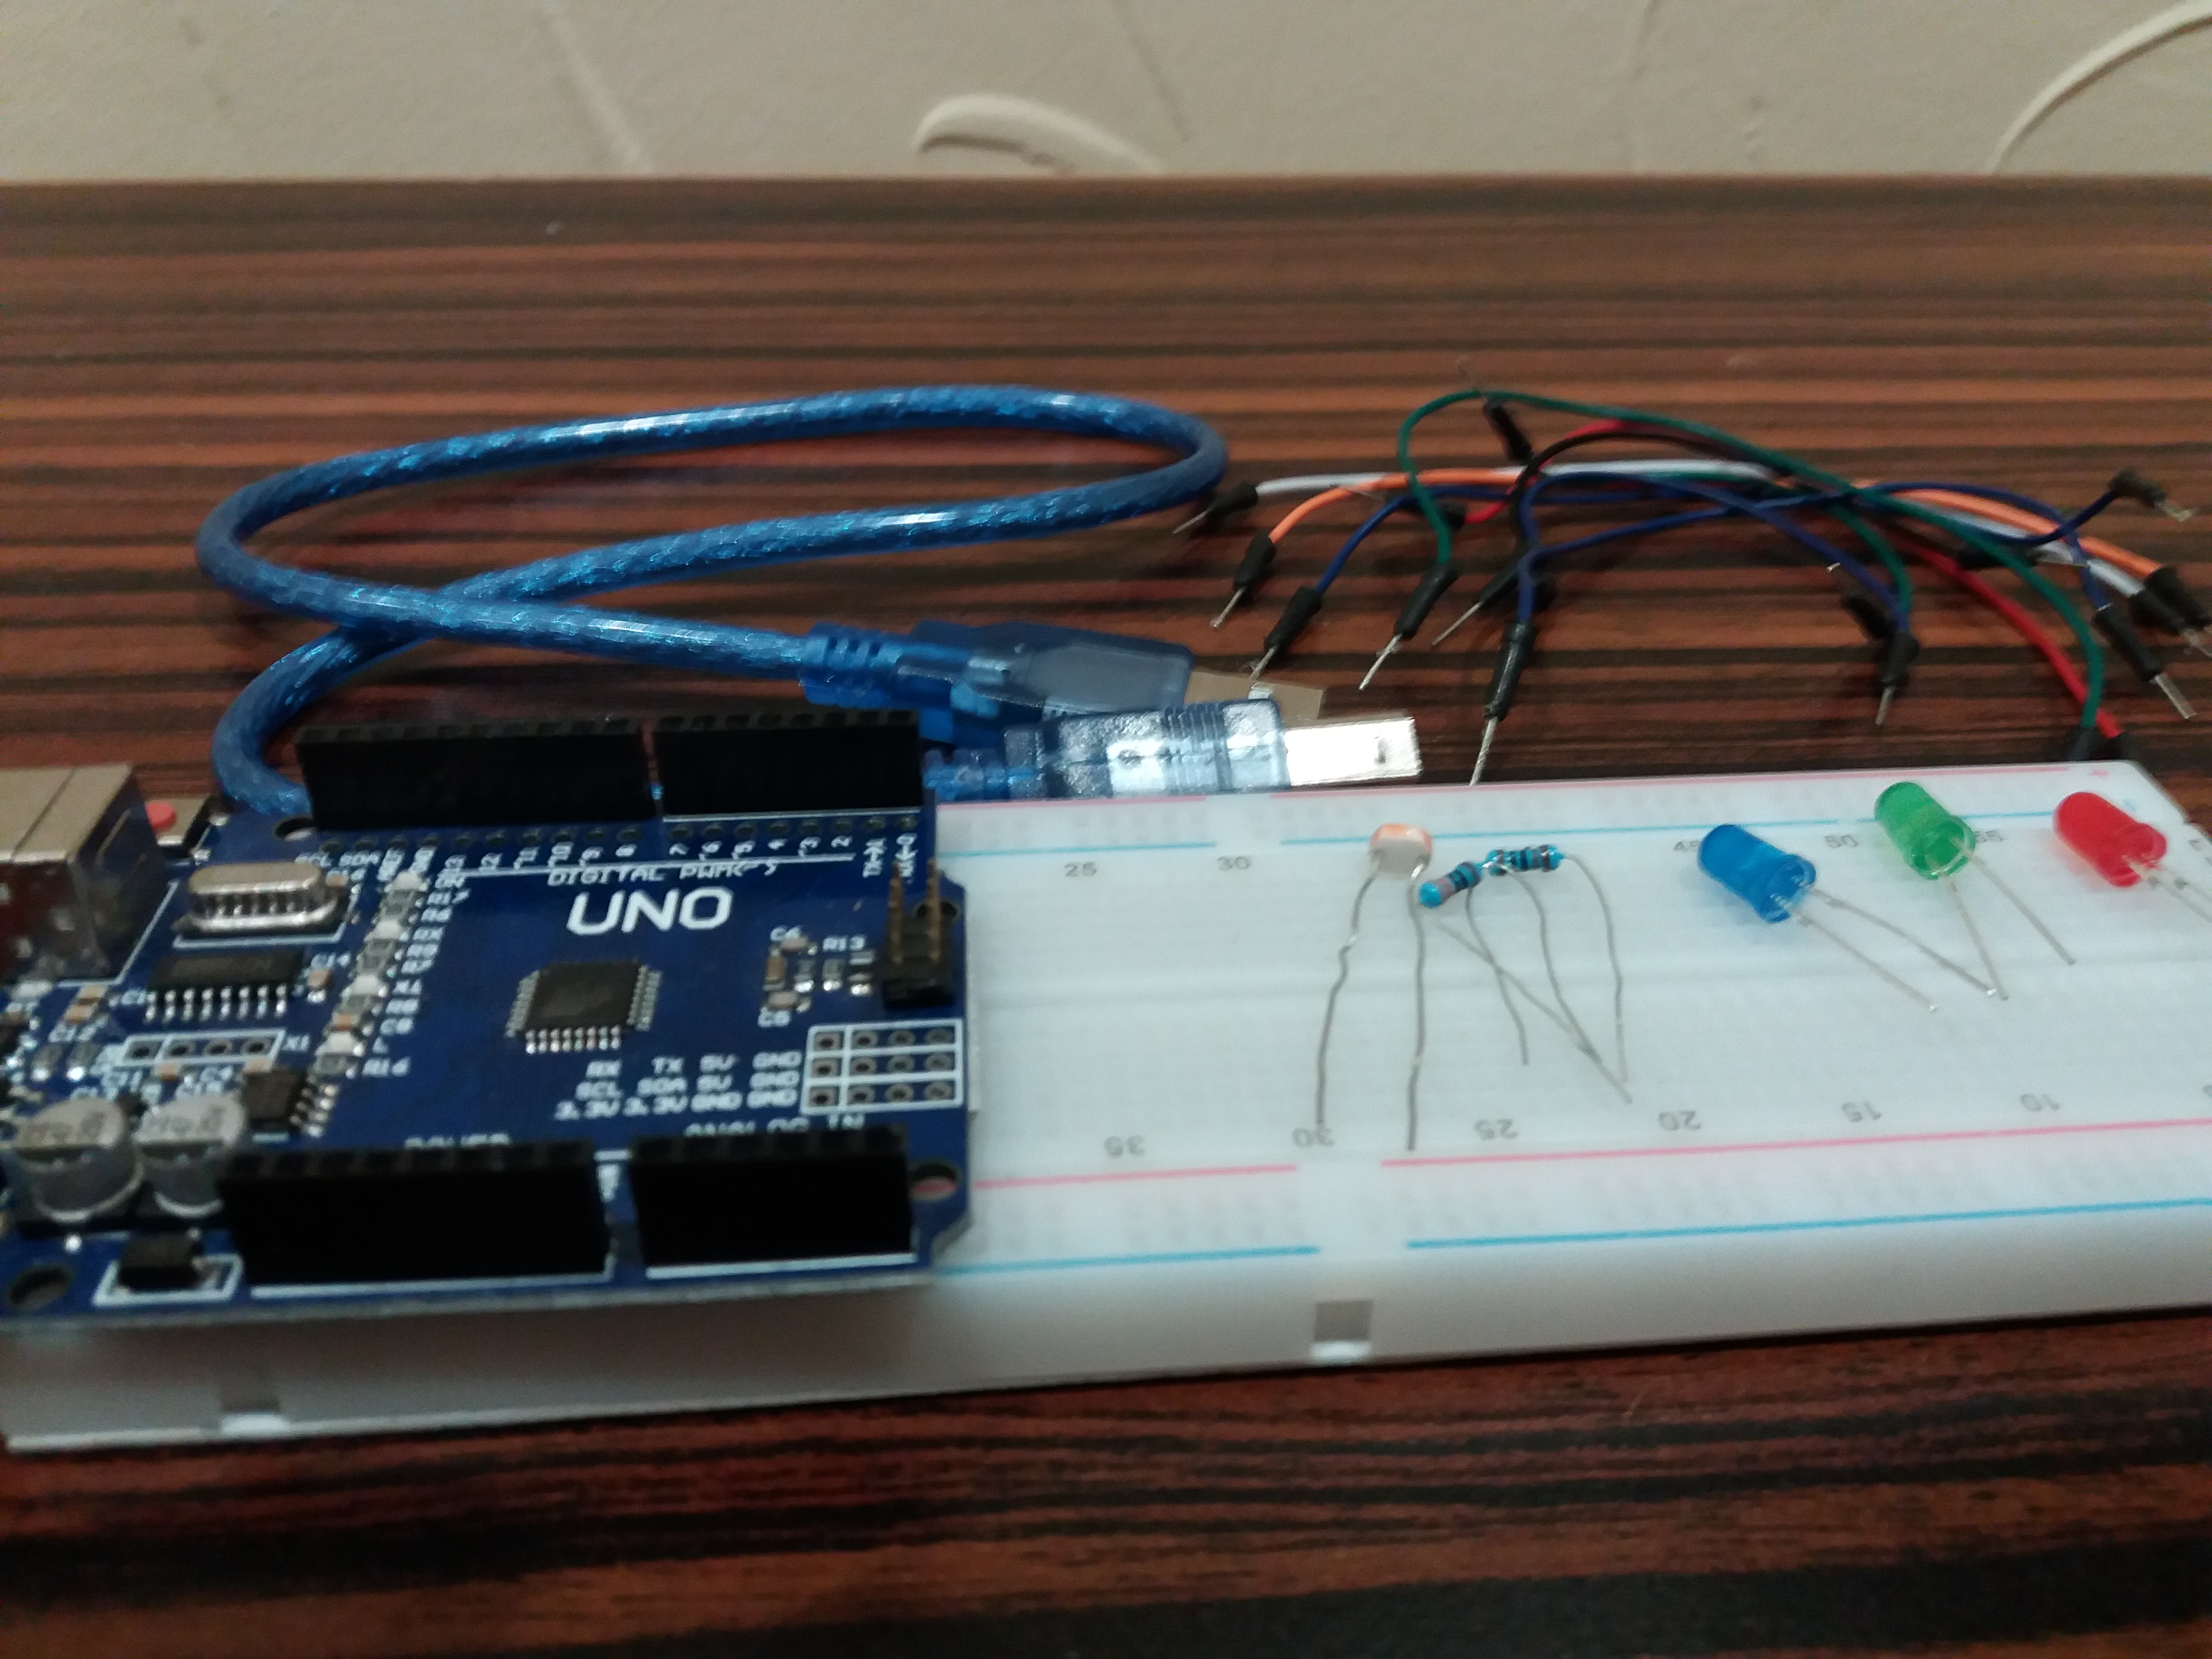
\includegraphics[width=8cm]{Capture1.jpg}
\captionof{figure}{equipments needed}
\end{center}

\item \textbf{Building the circuit} 

The reflected light from the emitter (RGB) LED bouncing back off of any objects will be read by the photosensor which will used calibrated values to find the individual R-G-B colour values of a particular colour.

To build the circuit we followed the following steps:

This will be the emitter part of our circuit emitting different colours which will bounce off of objects, by the law of optics which will be detected by our photosensor.

\begin{itemize}

\item We connected one end of each of the RGB coloured LED to pin 2, 3 and 4 respectively on the Arduino and the others to GND using the $1K\ohm$ resistor.

\item We connected one of the pins of the photosensor to the GND pin on the Arduino

\item We connected the second pin  of the photosensor to the 5V pin on the Arduino.

\item We connected also this second pin of the photosensor to the A0 pin on the Arduino: This is because we want to make a voltage divider to get the changing voltage reading as the reflected light changes in intensity.
\end{itemize}

The following figure shows the result of our wiring: 

\begin{center}
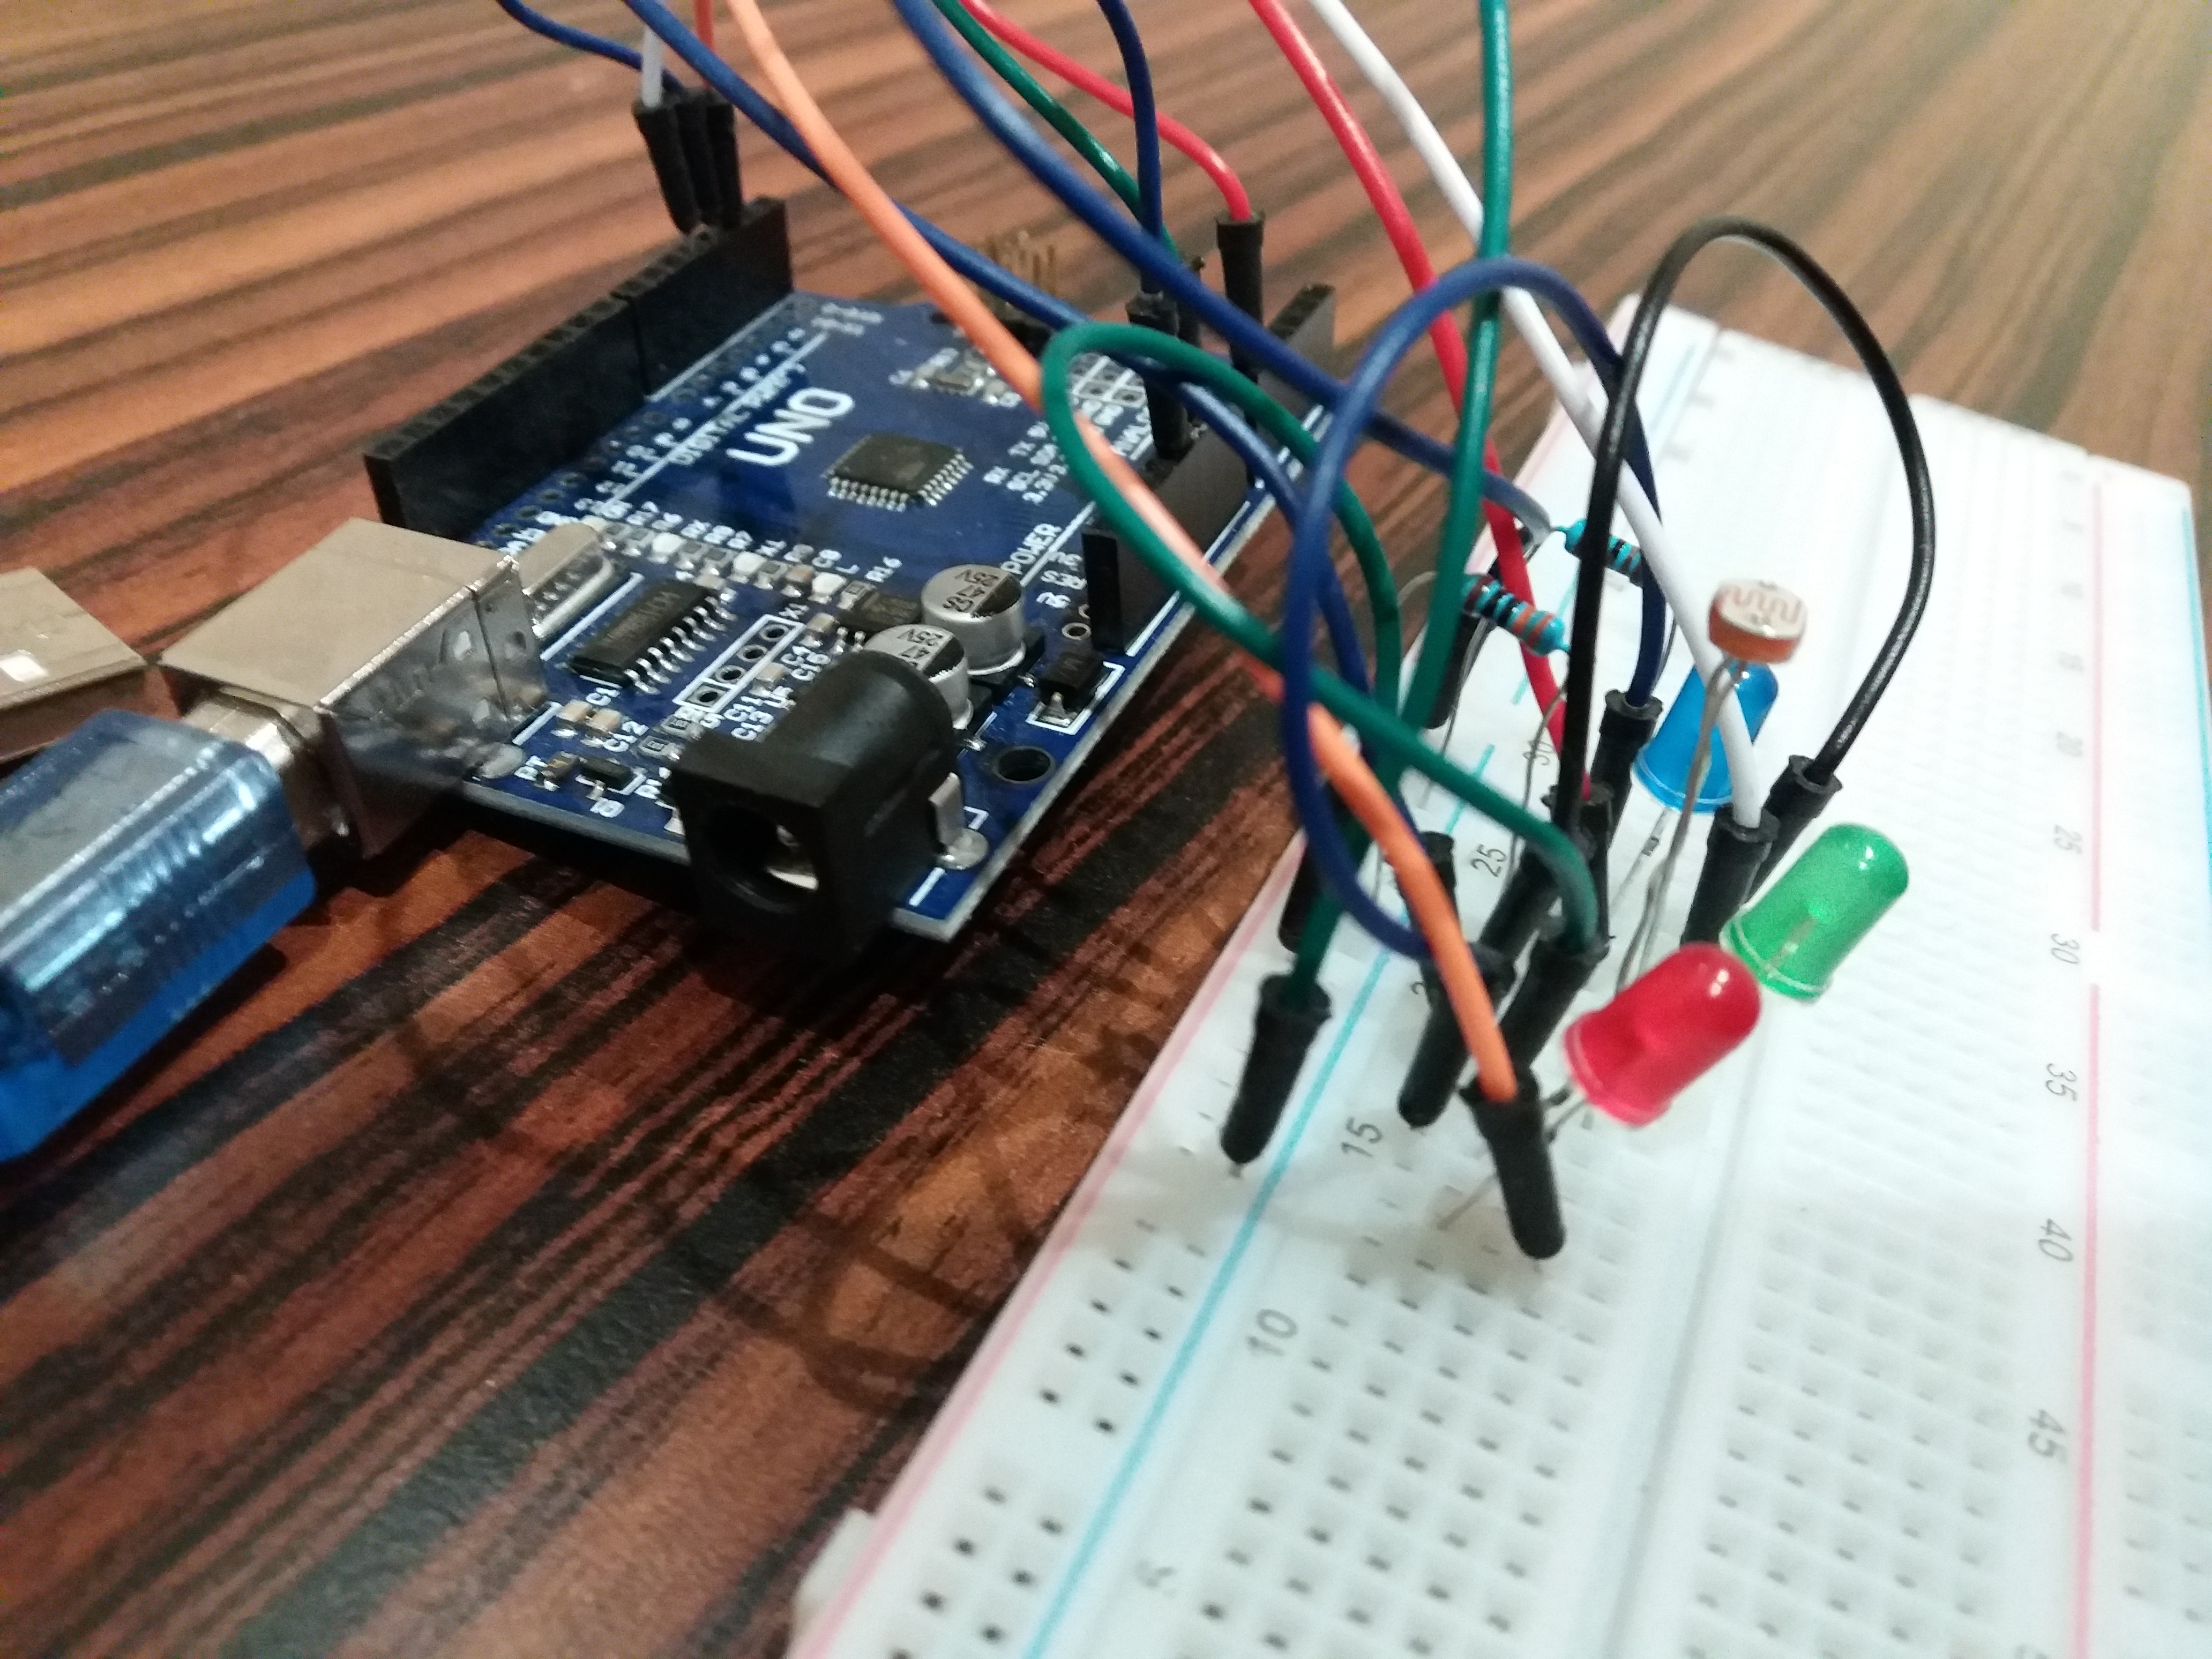
\includegraphics[width=8cm]{Capture2.jpg}
\captionof{figure}{Final circuit}
\end{center}

\item \textbf{Coding the Arduino}:

We implemented a simple code on the Arduino for creating the color sensor

\rule{18cm}{1pt} \\
Procedure:\\
\rule{18cm}{1pt} \\
\textbf{Input:} The reading from the sensor  

\textbf{Output:} Color detected on the screen  

\begin{enumerate}[\bf 1.]
\item initialization of the parameters
\item setup the Arduino
\item While true
\item \quad	\textbf{if} the balance the is not set (calibration set)
\item \quad \quad		\textbf{then} set balance 
\item \quad	\textbf{else}
\item 	\quad\quad	turn or the LEDs and read the color 
\end{enumerate} 

\item \textbf{Calibration}:
For that we need a black and white piece of paper before the uploading the code.

After uploading the code, we will have 5 seconds while the program running the RGB LED will emit a variety of colours to place a white paper over the LED and photosensor. Then we switch the paper to the white piece of paper for the next 5 seconds.

This will allow the code to correctly calibrate the sensor (255 for black and 0 for white)

\item \textbf{printing the colors with processing:}

For this we used a simple code  in Processing, it updates the background with the colour being sent out from the sensor, by placing diffrent colors in front of the sensor we can see that the screen show a very similar color


\subsection{Conclusion:}
In this work we were able to create a simple color sensor using RGB LEDs and a microcontroler ARDUINO , we were able to compare the color to be detected to the one printed on the screen and conclude that the sensor was able to give very good results in term of color resemblance 






\end{enumerate}
\end{document}	
